\documentclass[a4paper,10pt]{article}
%\usepackage[latin1]{inputenc} % Paquetes de idioma
\usepackage[utf8]{inputenc} % Paquetes de idioma (Este encoding toma acentos :) )
\usepackage[spanish]{babel} % Paquetes de idioma
\usepackage{graphicx} % Paquete para ingresar gráficos
\usepackage{grffile}
\usepackage{hyperref}
\usepackage{fancybox}
\usepackage{amsmath}
\usepackage{amsfonts}
\usepackage{listings}
\usepackage{float}
% Paquetes de macros de Circuitos
%\usepackage{pstricks}
\usepackage{tikz}

% Encabezado y Pié de página
\usepackage{fancyhdr} % Paquete para encabezados y pie de página
\pagestyle{fancy} % Sin esta línea no se imprimiría el encabezado en todas las páginas

\fancyhf{} %  Borra el encabezado anterior (Por defecto escribe el títutlo de la sección en la que se encuentra la hoja
\setlength{\headheight}{22.55pt}
\fancyhead[L]{
	{\textsf{Facultad de Ingenier\'ia $-$ Universidad de Buenos Aires \\ 66.44 Instrumentos Electrónicos}}
}
%\addtocounter{page}{5}
\fancyhead[R]{\thepage}

\renewcommand{\footrulewidth}{0.4pt} % Ajusta el tamaño de las líneas separadoras en el pié de página
\renewcommand{\headrulewidth}{0.4pt} % Ajusta el tamaño de las líneas separadoras en el encabezado

\fancyfoot[L]{
	{\textsf{Trabajo Pr\'actico N$^{\circ}4$}: Mediciones de impedancias} \\
	{\textsf{Integrantes: Eduardo Sanchez, Francisco Soler}}
	}
		

% Carátula del Trabajo
\title{ \author{} % Lo pongo para que el warning no moleste :p
\setlength{\unitlength}{1cm} %  Especifica la unidad de trabajo
\thispagestyle{empty}

\begin{picture}(18,0)
\put(0,0){
\includegraphics[width=1.5cm, height=3cm]{Logo1.png}}

\put(10.5,0){
\includegraphics[width=3cm, height=3cm]{Logo2.png}}

\end{picture}
\\[1.5cm]
\begin{center}
	\textbf{{\Huge Facultad de Ingenier\'ia \\ Universidad de Buenos Aires}}\\[2cm]
	{66.44 Instrumentos Electrónicos}\\[0.5cm]
	{Trabajo Pr\'actico N$^{\circ}3$: Mediciones de impedancias}\\[2.5cm]
\end{center}

\begin{flushleft}
	\textbf{Integrantes:} \\[1cm]

	\begin{tabular}{|c|c|c|}
		\hline
		\textbf{\normalsize Padr\'on} & \textbf{\normalsize Nombre} & \textbf{\normalsize Email} \\
		\hline
		\normalsize 92903 & \normalsize Sanchez, Eduardo Hugo & \normalsize hugo\_044@hotmail.com \\
		\hline
		\normalsize 91227 & \normalsize Soler, Jos\'e Francisco & \normalsize francisco.\_tw@hotmail.com \\
		\hline
		\normalsize xxx & \normalsize Wawrynczak, Claudio  & \normalsize claudiozak@gmail.com \\
		\hline
	\end{tabular}
\end{flushleft}
\date{} % Hace que no se imprima la fecha en la cual se compilo el .tex
 }

% \usepackage[disable]{todonotes} % notes not showed
\usepackage[draft]{todonotes}   % notes showed

% Select what to do with command \comment:  
% \newcommand{\comment}[1]{}  %comment not showed
\newcommand{\comment}[1]
{\par {\bfseries \color{blue} #1 \par}} %comment showed

\begin{document}
	\maketitle % Hace que el título anterior sea el principal del documento
	\newpage

	\tableofcontents % Esta línea genera un indice a partir de las secciones y 
					 % subsecciones creadas en el documento
	\newpage


\section{Objetivo}
\indent El objetivo de este trabajo consiste en implementar un mixer. Para ello 
se realiza un an\'alisis te\'orico del funcionamiento y de los par\'ametros 
m\'as relevantes de un mixer, para luego implementar un dise\~no propio. Al 
dise\~no propuesto se le realizan mediciones para caracterizarlo y documentar 
sus prestaciones.

\newpage
\subsection{Introducción teórica}
	\indent Un mixer de frecuencia es un circuito electrónico de 3 puertos. Dos
	de los mismos son entradas y el tercero se corresponde con la salida. El 
	mixer ideal mezcla ambas señales logrando así que la frecuencia de la señal 
	de salida sea la suma o la resta de las de las entradas, como se muestra en 
	la Ecuación \ref{eq:001}. La Figura \ref{img:001} muestra una representación
	gráfica del funcionamiento.
	
	\begin{equation}\label{eq:001}
		f_{out} = f_{in1} \pm f_{in2}
	\end{equation}

	\begin{figure}[!htb]
		\centering
		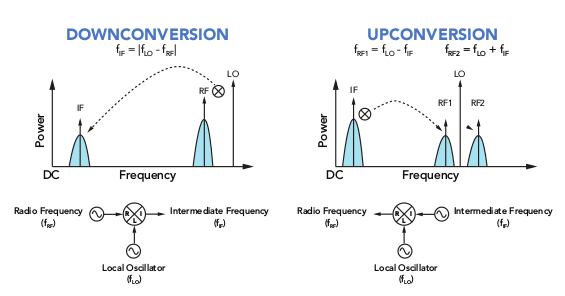
\includegraphics[width=10cm]
		{Images/MixerFunction.png}
		\caption{Suma y resta de frecuencias en un mixer ideal}
		\label{img:001} 
	\end{figure}

	\indent La nomenclatura de los puertos son:
	\begin{itemize}
		\item Local Oscillator (LO)
		\item Radio Frequency (RF)
		\item Intermediate Frequency (IF)
	\end{itemize}

	\indent La señal que ingresa en el puerto LO funciona como gate del mixer 
	en el sentido que el mixer puede considerarse ``ON'' cuando dicha señal está
	en alto y en ``OFF'' cuando está en estado bajo, este puerto solo puede ser 
	utilizado como entrada. \\
	\indent Los otros dos puertos del mixer, IF y RF, pueden intercambiarse 
	dependiendo de que es lo que se busque. Si se utiliza al puerto IF como 
	entrada, se logra obtener la suma de frecuencias, si la entrada es 
	el puerto RF, se obtiene la resta de frecuencias. La relación entre la 
	entrada y salida de frecuencias se muestra en la Ecuación \ref{eq:002}

	\begin{equation}\label{eq:002}
		f_{IF} = |f_{LO} - f_{RF}|
	\end{equation}
%	\todo[inline]{si se queda con la resta no se llama downconverter y si se queda con la suma es upconverter??
%	sisi, la resta es downconverter, la suma es upconverter, si mal no recuerdo
%	... me gusta que hayas comenzado a utilizar los todos ;)}
	\indent En la Figura \ref{img:001}, que representa ambas configuraciones de 
	funcionamiento, se puede observar que en el caso de upconversion se observa
	la suma y resta de frecuencias. Si se observan ambas se la llama 
	upconversion de doble ancho de banda. Es posible armar uno de ancho de banda
	simple, en este caso la suma o la resta de frecuecias es intencionalmente 
	cancelada dentro del mixer. Dichos dispositivos se los llama single sideband
	modulators. \\
	\indent En principio, cualquier componente no lineal puede ser utilizado 
	para armar un mixer; actualmente se utilizan diodos schottky, transistores 
	GaAs FETs y CMOS. La elección depende de la aplicación. Los mixers FET y 
	CMOS se utilizan cuando la performance es menos importante y el costo es 
	crucial. Para aplicaciones de alta performance se utilizan mixers de didos 
	schottky.
	
	\begin{figure}[!htb]
		\centering
		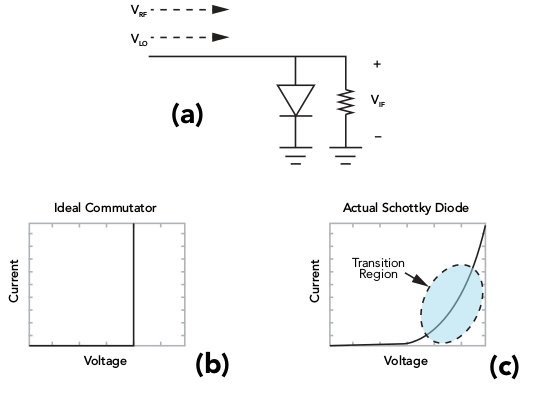
\includegraphics[width=10cm]
		{Images/OneDiodeMixer.png}
		\caption{(a) Mixer de un diodo. características I-V para (b)
		conmutador ideal y (c) diodo schottky real.}
		\label{img:002} 
	\end{figure}

	\begin{figure}[!htb]
		\centering
		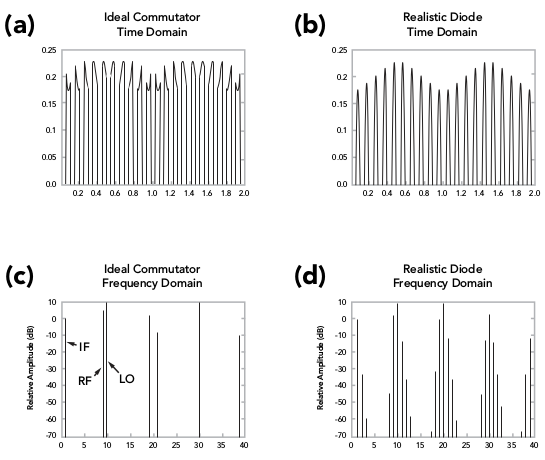
\includegraphics[width=10cm]
		{Images/OneDiodeMixerFunction.png}
		\caption{Comparaci\'on de la salida de un mixer de un diodo en el 
		dominio del tiempo y frecuencia con características de switching 
		de diodos ideales y reales} 
		\label{img:003} 
	\end{figure}


	\subsubsection{Mixer de un diodo: Conmutador ideal vs diodo real}
	\indent El mixer más simple consiste en un único diodo, como se muestra en 
	la Figura \ref{img:002}a. Se utiliza una gran señal de LO y otra pequeña de 
	RF combinadas en el ánodo del diodo. En el enfoque ideal, como la señal del 
	LO es dominante, la transconductancia del diodo es solo afectada por la 
	misma. A su vez, se asume que el diodo switchea instantáneamente como se 
	muestra en la Figura \ref{img:002}b. Dispositivos que cumplen con lo 
	anteriormente mencionado se los llaman conmutadores ideales y poseen la 
	máxima performance como mixer. \\
	\indent El proceso de mezclado se produce debido a la respuesta del diodo 
	con respecto a la señal LO. Debido a que diodo es forzado a circuito abierto 
	y cerrado por la señal LO, la señal pequeña de RF es chopeada. Si se 
	analizan las componentes de Fourier de la señal de salida de la conmutación 
	de dicho mixer (ver Figuras \ref{img:003}a y \ref{img:003}c), se observa que
	cumple con la siguiente relación:

	\begin{equation*}
		f_{IF} = n\cdot f_{LO}\pm f_{RF}~(n\text{impar})
	\end{equation*}

	\indent Por ende, en el caso ideal de un conmutador de switcheo, solo los 
	armónicos impares del LO se mixean con el tono fundamental de RF. \\
	\indent Como dicha función transferencia nunca puede alcanzarse en el caso 
	real, hay un tiempo de transición del estado bajo a uno alto (como se 
	muestra en la Figura \ref{img:002}c), la señal RF tambi\'en modula la 
	transconductancia de los diodos en algún porcentaje. La combinación de las 
	características reales de los diodos y la modulación de la transconductancia
	causan todos los componentes de armónicos de la señal IF. Las Figuras 
	\ref{img:003}b y \ref{img:003}d muestran la señal de salida en tiempo real y
	el equivalente en el dominio de la frecuencia. Matemáticamente, los 
	componentes de frecuencias generados por un diodo solo se muestran en la 
	Ecuación \ref{eq:003}

	\begin{equation}\label{eq:003}
 		f_{IF} = n f_{LO}\pm m f_{RF}~(\text{m y n enteros})
	\end{equation}

	\indent Como solo se desea una única frecuencia de salida (cuando n y m = 1)
	, eliminar todos los armónicos es el objetivo principal de un buen diseño 
	de un mixer. Este análisis muestra los siguientes atributos de los mixers de
	frecuencia:

	\begin{itemize}
		\item La mezcla se produce por el comportamiento de switcheo del diodo.
		\item La mayoría de los armónicos no deseados son generados por la 
		intermodulación no lineal de las señales de RF y LO en la región de 
		transmisión del diodo.
		\item Los mejores mixers utilizan diodos que se aproximan al conmutador 
		ideal.
		\item Mientras menor sea la potencia de la señal RF, la presencia de 
		espurios disminuye (dado que la señal del LO controlará la 
		transconductancia del diodo de forma más efectiva).
	\end{itemize}

	\subsubsection{Mixer balanceados}
	\indent Uno de los problemas que genera utilizar un único diodo como mixer 
	es que el LO debe radiar parte de la potencia de entrada desde el puerto de 
	entrada, esto genera una sensibilidad menor, que la potencia de salida 
	disminuya aún mas y la generación de frecuencias espurias en la salida por 
	mixeos entre armónicos. \\
	\indent Como consecuencias surgen los mixers balanceados, este nombre no 
	viene dado por la cantidad de diodos que poseen, sino por la cantidad de 
	espurios que quedan en la señal resultante, balanceados 50\% y doble 
	balanceados 25\%. \\
	\indent Normalmente un mixer doblemente balanceado utiliza cuatro diodos en 
	una configuración de anillo o estrella. Cada puerto del mismo permanece
	aislado del resto. Las ventajas de uno doblemente balanceado frente a uno 
	simple son las siguientes:
	
	\begin{itemize}
		\item Aumenta la linealidad
		\item Mejora la supresión de espurios
		\item Se incrementa la aislación entre puertos
		\item Posee un ancho de banda superior
	\end{itemize}

	\indent En contraposición, las desventajas son

	\begin{itemize}
		\item Se requieren dos transformadores balun
		\item Se requiere una mayor potencia de señal LO
		\item Posee menor ganancia
		\item La frecuencia de corte superior es menor
	\end{itemize}

	\indent La Figura \ref{img:004} muestra un diagrama de un mixer doblemente 
	balanceado. El funcionamiento se puede explicar mejor si se consideran los 
	diodos como switches. \\
	
	\begin{figure}[!htb]
		\centering
		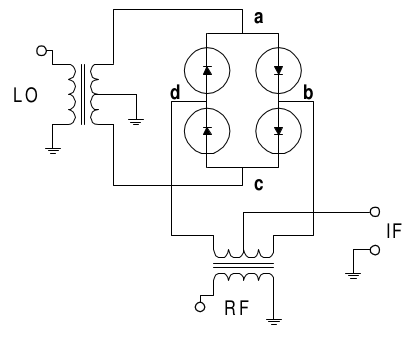
\includegraphics[width=8cm]{Images/DoubleBalancedMixer.png}
		\caption{Mixer doblemente balanceado}
		\label{img:004}
	\end{figure}

	
	\indent El LO abre y cierra cada rama del puente de diodos de
	forma alternada, cada rama está en contrafase. Los puntos ``a'' y ``c'' son 
	tierras virtuales con respecto a la señal entrante de RF. Por lo tanto, ``b'' 
	y ``d'' (la señal RF balanceada) es alternadamente conectada a tierra (puntos 
	``a'' y ``c''). Esto significa que las parte de la señal RF en fase y anti fase 
	con respecto al LO es alternadamente conectada a la tierra. Por lo tanto, la
	señal en el puerto IF es efectivamente la señal RF multiplicada por una 
	señal cuadrada de magnitud pico $\pm 1$ y frecuencia LO. \\
	
	\begin{figure}[!htb]
		\centering
		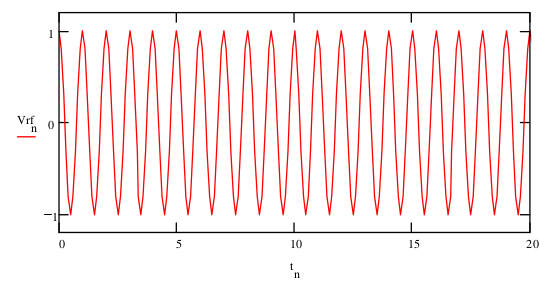
\includegraphics[width=8cm]{Images/VRF.png}
		\caption{Señal del RF, tensión vs tiempo en nseg}
		\label{img:005}
	\end{figure}

	\indent La Figura \ref{img:005} muestra una señal senoidal de 1GHz en el
	puerto RF. La Figura \ref{img:006} muestra una señal cuadrada en una 
	frecuencia de 870MHz, es la señal de switching del puerto LO. La 
	multiplicación resultante (en el puerto IF) es mostrada en la Figura 
	\ref{img:007}, y, como se puede observar, posee una frecuencia de 130MHz. \\
	
	\begin{figure}[!htb]
		\centering
		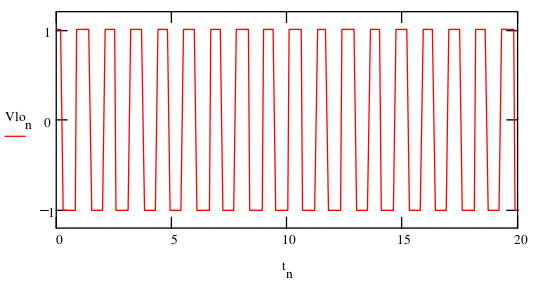
\includegraphics[width=8cm]{Images/VLO.png}
		\caption{Señal del LO, tensión vs tiempo en nseg}
		\label{img:006}
	\end{figure}
	
	\indent Si bien este análisis explica a grandes razgos como funciona el 
	mixer, no es adecuado para determinar las pérdidas del mismo, dado que, si 
	se utilizara una cuadrada ideal, dicho proceso debería tener una conversion
	loss de 3.9 dB. En la práctica ronda en los 6 a 8 dB, debido a las pérdidas
	de los diodos, los transformadores, etc. \\
	
	\begin{figure}[!htb]
		\centering
		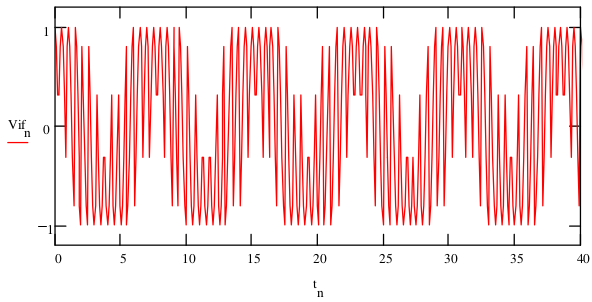
\includegraphics[width=8cm]{Images/VIF.png}
		\caption{Tension de IF (Vrf*Vlo) versus tiempo en nseg}
		\label{img:007}
	\end{figure}

	\indent En la Figura \ref{img:004} se utilizan transformadores con ferrites 
	para generar las señales RF y LO diferenciales. Dichos transformadores 
	pueden ser utilizados hasta 1-2 GHz, para frecuencias mayores ya se deben 
	reemplazar por líneas de transimisión. En este caso se elgieron los 
	ferrites toroidales FT37-67, que, según la especificación, llegan hasta 1GHz
	como transformadores. Otro tipo de ferrite es el balun que tambi\'en posee las
	mismas especificaciones, pero como no se consiguieron se utilizaron los 
	primeros.\\
	\indent Hay que tener en cuenta, que para bobinar dicho ferrite, hay que 
	twistear los cables, en este caso en particular son de a tres cables a la 
	vez y dos de ellos conforman el secundario del transformador.

\newpage
\section{Desarrollo}
	\subsection{Parámetros de un mixer}
	En esta secci\'on se explica detalladamente cada uno de los par\'ametros del mixer y c\'omo puede medirse, para realizarlo luego en el dise\~no propuesto.
		\subsubsection{Impedancias de entrada y salida}
		Es la impedancia que presentan los puerto RF e IF, generalmente est\'an estandarizados a $50\Omega$ para determinado rango de frecuencias. Para estos par\'ametros resulta conveniente utilizar el analizador de redes para medir el valor de la impedancia as\'i como su respuesta en frecuencia.
		\subsubsection{P\'erdidas por conversi\'on}
		\indent La eficiencia del mixer se mide de acuerdo a las p\'erdidas por conversi\'on (conversion loss, en ingl\'es), es decir, la 
		relación entre la potencia de la señal del puerto RF con respecto a la potencia de la señal del puerto IF. Matem\'aticamente esto es,
		$$\textmd{P\'erdidas por conversi\'on}=10\cdot\log\left(\frac{P_{RF}}{P_{IF}}\right)$$
		Evidentemente se busca que \'este tenga un valor bajo, ya que no se desea gastar potencia en exceso. Valores t\'ipicos de p\'erdidas por conversi\'on son de $4.5~dB$ a $9~dB$, debido a las p\'erdidas en las l\'ineas de transmisi\'on, la resistencia serie de los diodos, desajustes en los transformadores, entre otros.
		Una forma sencilla de medir este par\'ametro es colocar en el puerto RF una señal de potencia conocida (proporcionada por un sintetizador de frecuencias, por ejemplo) y utilizando un analizador de espectro observar la potencia de la señal del puerto IF.
		
		\subsubsection{Aislación entre puertos}
		La aislación entre puertos es una medida de la cantidad de potencia que se ``fuga'' de un puerto a otro puerto del mixer.
		En particular interesan tres aislaciones:
		\begin{itemize}
		\item Del puerto LO al puerto IF
		\item Del puerto LO al puerto RF
		\item Del puerto RF al puerto IF
		\end{itemize}
		La aislaci\'on se mide de la siguiente manera: dada una se\~nal de potencia $P_{in}$ en el puerto LO (o RF, depende de qu\'e aislaci\'on se desee obtener), con un analizador de espectro se observa la potencia, $P_{out}$, de la señal del puerto RF (o IF) a la frecuencia de la señal que se encuentra en el puerto LO (o RF). De esta manera la aislaci\'on se calcula como		$$\textmd{Aislaci\'on}=10\cdot\log\left(\frac{P_{in}}{P_{out}}\right)$$
		Es importante notar que cada puerto que no se utilice en la medici\'on deben estar terminado en una impedancia de funcionamiento real.
		
		Por otra parte, cuando se especifica la aislaci\'on de un mixer, \'esta debe realizarse sobre una banda de frecuencias. Con lo cual resulta m\'as pr\'actico medirlo utilizando el analizador de redes, prestando especial atenci\'on a los niveles de potencia utilizados para medir en el mixer.
		\subsubsection{Componentes espurias}
		Como en todo dispositivo electr\'onico, el mixer presenta algunas alinealidades con lo cual adem\'as de la presencia de la frecuencia de inter\'es ($f_{IF}=f_{RF}-f_{LO}$), est\'an presentes otras componentes espectrales ($f_{espurias}=m\cdot f_{RF}-n\cdot f_{LO}$ con $m$ y $n$ enteros). Se especifica como la diferencia (en dB) entre la amplitud de la frecuencia $f_{IF}$ y la amplitud de las componentes espurias. Se especifica para una frecuencia y nivel de potencia determinados de la señal del puerto LO.
		Esta especificaci\'on puede obtenerse midiendo con un analizador de espectro las amplitudes de la frecuencia $f_{IF}$ y de las frecuencias espurias $f_{espurias}$.

		\subsubsection{Figura de ruido}
		\indent La figura de ruido es otra medición para ver la eficiencia del 
		mezclado. Es la relación de la señal ruido de la entrada con respecto a
		la señal ruido de la salida. Es decir
		
		$$F=\frac{\frac{S_i}{N_i}}{\frac{S_o}{N_o}}$$
		La cual puede re-escribirse de la siguiente manera expres\'andola en decibeles 
		$$F=10\cdot\log\left(\frac{S_i}{S_o}\cdot\frac{N_o}{N_i}\right)$$
		Y usando la definici\'on de p\'erdidas por conversi\'on, finalmente queda
		$$F=\textmd{P\'erdidas por conversi\'on}+10\cdot\log\left(\frac{N_o}{N_i}\right)$$
		Donde la potencia $N_o$ puede obtenerse utilizando el analizador de redes.
		
		\subsubsection{Compresi\'on de conversi\'on}
		La compresi\'on de conversi\'on es una medida del m\'aximo nivel de se\~nal para la cual el mixer proporciona una operaci\'on lineal. A bajos niveles de potencia de la se\~nal del puerto RF, las p\'erdidas por conversi\'on son constantes. No obstante, cuando la potencia de la se\~nal del puerto RF est\'a aproximadamente dentro de los 10 dB del nivel de potencia de la se\~nal del puerto LO, la potencia de la se\~nal del puerto IF no sigue los aumentos de potencia de la se\~nal del puerto RF. Con lo cual las p\'erdidas por conversi\'on empiezan a aumentar pasado este nivel de potencia en el puerto RF. El criterio usado para medir la desviaci\'on respecto del funcionamiento lineal del mixer es el siguiente: cuando las p\'erdidas por conversi\'on son 1 dB m\'as grandes que cuando se trabaja con niveles bajos de potencia, se alcanza el m\'aximo nivel de se\~nal del puerto RF permitido. Con el analizador de espectro se puede ir observando la se\~nal del puerto IF y observar cuando tiene una diferencia extra de 1 dB con la se\~nal del puerto RF. 
		
		\subsubsection{Rango din\'amico}
		El rango din\'amico del mixer es el rango de potencias de se\~nal en el puerto RF para el cual el mixer proporcional un funcionamiento \'util.
		El punto de compresi\'on de conversi\'on acota superiormente el rango din\'amico y la figura de ruido acota inferiormente el rango din\'amico por lo cual queda \'este queda especificado por las mediciones previas.

		\subsubsection{DC Offset}
		Es una medida del desbalance del mixer. Para un mixer perfectamente balanceado el offset de continua es cero.


	\section{Diseño a armar}
	\indent Dado que se el mixer opera a frecuencias altas, al momento de dise\~nar la placa deben tenerse en cuenta determinados criterios. Las pistas del impreso deben ser cortas y gruesas, debe evitarse formar lazos de cobre que eventualmente acoplen interferencias, los \'angulos de 90 grados en las pistas deben eliminarse ya que esto genera una desadapaci\'on de impedancias y por lo tanto ondas reflejadas en dicho nodo, entre otros. Teniendo en cuenta estos criterios se realiz\'o el PCB del mixer como se puede observar en la Figura \ref{pcb}.
	
	\indent Respecto de los componentes utilizados en la placa se tuvieron en cuenta las siguientes cuestiones:
	\begin{itemize}
	\item Los diodos Schottky utilizados deben ser de baja capacidad de juntura para poder operar a un rango de frecuencias elevado como el que se pretende. Por ello se eligieron los diodos BAT85 de $C_j=10~pF$, el valor m\'as bajo que pudo obtenerse. 
	\item Los transformadores se realizaron con ferrites de alta frecuencia bobinados con cable de cobre esmaltado de ??mm. El cable que bobina cada ferrite es un cable trifilar, un hilo que corresponde al primario y otros dos hilos que corresponden al secundario del transformador.
	\item Los conectores utilizados para los puertos RF, IF y LO son conectores BNC, cuyo rango de operaci\'on, hasta aproximadamente $4~GHz$, es suficiente para el fin buscado.
	\item La placa es Epoxi m\'as adecuada que las Pertinax para altas frecuencias.
	\item Cuenta con un gabinete m\'etalico que le otorga blindaje electromagn\'etico frente a interferencias externas.
	\end{itemize}
	 
	\begin{figure}[!htb]
		\centering
		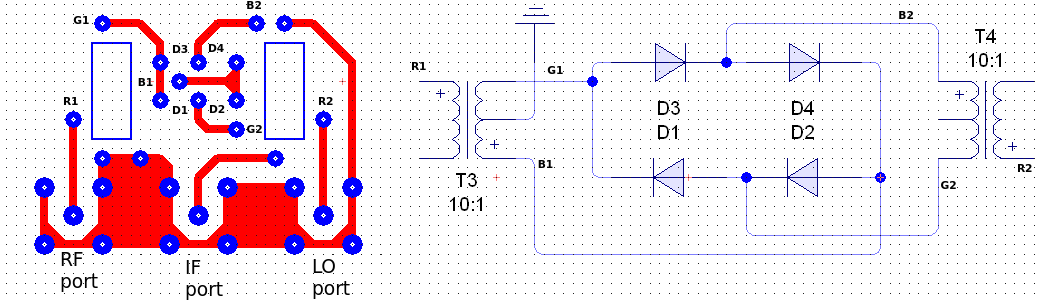
\includegraphics[width=8cm]{Images/PCB.png}
		\caption{PCB}
		\label{pcb}
	\end{figure}
	
	Finalmente en la Figura \ref{ecuadorputa} se puede ver el dise\~no del mixer terminado. 
	
		\begin{figure}[!htb]
			\centering
			\includegraphics[width=8cm]{Images/gabi.png}
			\caption{Mixer}
			\label{ecuadorputa}
		\end{figure}
%	\section{Mediciones}
%	\todo[inline]{ojala sea este fuckiiiing martes :D}
%	\subsubsection{Impedancias de entrada y salida}
%	\subsubsection{P\'erdidas por conversi\'on}
%	\subsubsection{Aislación entre puertos}
%	\subsubsection{Componentes espurias}
%	\subsubsection{Figura de ruido}
%	\subsubsection{El punto de compresi\'on de conversi\'on}
%	\subsubsection{Rango din\'amico}
%	\subsubsection{DC Offset}
%	\newpage
%	\section{Conclusiones}
%	\indent Vamos Argentinaaaaa!!!
\end{document}
